
%(BEGIN_QUESTION)
% Copyright 2012, Tony R. Kuphaldt, released under the Creative Commons Attribution License (v 1.0)
% This means you may do almost anything with this work of mine, so long as you give me proper credit

A high-voltage circuit breaker is manually operated from a remote location using a pair of pushbutton switches, connected to ``trip'' and ``close'' solenoid coils within the breaker:

$$\includegraphics[width=15.5cm]{i02111x01.eps}$$

This particular circuit breaker is gas-quenched by sulfur hexafluoride gas (SF$_{6}$), which is normally pressurized inside the circuit breaker to approximately 45 PSI for optimum electrical performance.  

\vskip 10pt

A low-pressure lockout switch is being installed on the circuit breaker to detect if the SF$_{6}$ gas pressure ever drops below 35 PSI.  The purpose of this switch is to disable the breaker from either closing or tripping if the gas pressure is abnormally low.

Your task is to modify the circuit shown above to include this pressure switch.  The single-pole, double-throw pressure switch is shown in the upper-right corner of the diagram, not yet connected to the 125 VDC trip/close circuit.

\vfil 

\underbar{file i02111}
\eject
%(END_QUESTION)





%(BEGIN_ANSWER)

This is a graded question -- no answers or hints given!

%(END_ANSWER)





%(BEGIN_NOTES)

In order for the low-pressure lockout switch to perform its intended function, it must prevent any 125 VDC power from getting to either trip or close coils in the circuit breaker.  This suggests placing the lockout switch in series with everything so that it may disable both the trip and close functions by opening.

If we wish this pressure switch to open under low-pressure conditions, we must wire it in such a way that its resting state (its ``normal'' state according to the manufacturer) will be open, since the ``normal'' state for a pressure switch is when no pressure is applied to it at all.  This way, an unusually low gas pressure inside the circuit breaker will cause the switch to go toward its resting state, opening up, and preventing power from ever reaching either actuating coil inside the breaker.

\vskip 10pt

This is one possible solution:

$$\includegraphics[width=15.5cm]{i02111x02.eps}$$

%INDEX% Electric power systems: HV circuit breaker controls

%(END_NOTES)


